\section{System Architecture}

\subsection{Architecture Overview}
The application architecture is structured on three foundational engineering pillars: Robert C. Martin's \textbf{Clean Architecture}, \textbf{Manual Dependency Injection (DI)} via an \texttt{AppContainer} composition root, and the \textbf{Model-View-ViewModel (MVVM)} pattern coupled with \textbf{Unidirectional Data Flow (UDF)} in the presentation layer.

\subsubsection{Clean Architecture Rationale}
In mobile applications integrating rapidly advancing Artificial Intelligence and Machine Learning (AI/ML) capabilities, system requirements and external dependencies shift frequently: a cloud API endpoint may change, a local neural network model may be upgraded, or a new indexing strategy may be tested. Adopting Clean Architecture guarantees:
\begin{enumerate}
    \item \textbf{Complete Independence from External Frameworks:}
    The core business layer (\textbf{Domain Layer}) is implemented in pure Kotlin. Use cases such as \texttt{AnalyzeDocument}, \texttt{SearchDocuments}, and \texttt{SaveDocument} maintain zero dependencies on Android SDK classes or specific ML libraries. They interact exclusively through abstract interfaces (\texttt{DocumentRepository}, \texttt{OcrService}, \texttt{EmbeddingService}, \texttt{LlmService}).
    
    \item \textbf{Pluggable and Interchangeable Service Implementations:}
    Transitioning from a cloud-based multimodal model (Gemini Vision API) to an on-device pipeline (ML Kit OCR + MediaPipe Summarizer) requires merely swapping the concrete implementation in the composition root without altering a single line of business or UI code.
    
    \item \textbf{High Automated Testability:}
    Business rules, search ranking algorithms, and similarity metrics can be validated via fast JVM unit tests using lightweight test doubles (e.g., \texttt{FakeDocumentDao}, \texttt{FakeEmbeddingService}) without requiring an Android emulator or physical hardware.
    
    \item \textbf{Strict Separation of Concerns:}
    Presentation, Domain, and Data logic remain strictly isolated, simplifying collaborative git branching and preventing spaghetti dependencies.
\end{enumerate}

\subsubsection{Dependency Injection with \texttt{AppContainer}}
Rather than relying on heavy compile-time annotation processors such as Dagger-Hilt (which introduce significant build latency and verbose generated code), the project utilizes a clean \textbf{Manual Dependency Injection} pattern anchored by \texttt{AppContainer}:
\begin{itemize}
    \item \texttt{AppContainer} instantiates and manages the lifecycles of singleton dependencies: the local Room Database (\texttt{AppDatabase}), the image storage service, ML services (ML Kit, MediaPipe), and the Gemini API client.
    \item It wires concrete dependencies into Domain Use Cases (\texttt{ObserveDocuments}, \texttt{SearchDocuments}, \texttt{SaveDocument}, etc.).
    \item It exposes customized \texttt{ViewModelProvider.Factory} instances, ensuring that ViewModels receive only the precise use cases necessary for their execution.
\end{itemize}

\subsubsection{Presentation Architecture}
\begin{itemize}
    \item \textbf{View (Composables):} Built declaratively using Jetpack Compose. Views observe an immutable state (\texttt{UiState}) emitted by the ViewModel and propagate user interactions as explicit actions/events.
    \item \textbf{ViewModel:} Extends \texttt{androidx.lifecycle.ViewModel}, hosts a backing \texttt{MutableStateFlow<UiState>}, executes asynchronous workflows via Kotlin Coroutines, and updates the observable UI state.
    \item \textbf{Unidirectional Data Flow (UDF):} State flows downward from ViewModel to Composable screens; user events flow strictly upward from Composables into ViewModel entry points, preventing UI race conditions.
\end{itemize}

\subsection{Architecture-to-Project Mapping}

The three concentric Clean Architecture tiers map directly to the codebase package structure:

\begin{table}[H]
\centering
\small
\begin{tabularx}{\textwidth}{l p{4.5cm} X}
\toprule
\textbf{Layer} & \textbf{Core Components} & \textbf{Project Location} \\
\midrule
\textbf{Presentation} & Compose Screens, ViewModels, UI State definitions, Navigation & 
\texttt{presentation/capture/} \newline
\texttt{presentation/review/} \newline
\texttt{presentation/library/} \newline
\texttt{presentation/detail/} \newline
\texttt{presentation/setting/} \newline
\texttt{navigation/AppNavGraph.kt, Routes.kt} \\
\midrule
\textbf{Domain} & Entities, Domain Models, Use Cases, Service Contracts & 
\texttt{domain/model/} \newline
\texttt{domain/usecase/} \newline
\texttt{domain/service/} \newline
\texttt{domain/repository/} \\
\midrule
\textbf{Data} & Room Database, DAO, Entity Mappings, ML Adapters & 
\texttt{data/local/} \newline
\texttt{data/repository/} \newline
\texttt{data/ml/} \\
\bottomrule
\end{tabularx}
\caption{Detailed architectural component and package directory correlation}
\label{tab:arch_mapping}
\end{table}

\subsection{System Execution Flows}
The following sequence diagrams illustrate the runtime coordination among layers during core user journeys (extracted from \texttt{docs/DIAGRAMS.md}):

\subsubsection{Document Processing Flow}
The sequence below demonstrates image capture, automatic metadata generation (Gemini Vision or On-Device fallback), presentation of the interactive Review screen, and embedding computation upon user confirmation:

\begin{figure}[H]
\centering
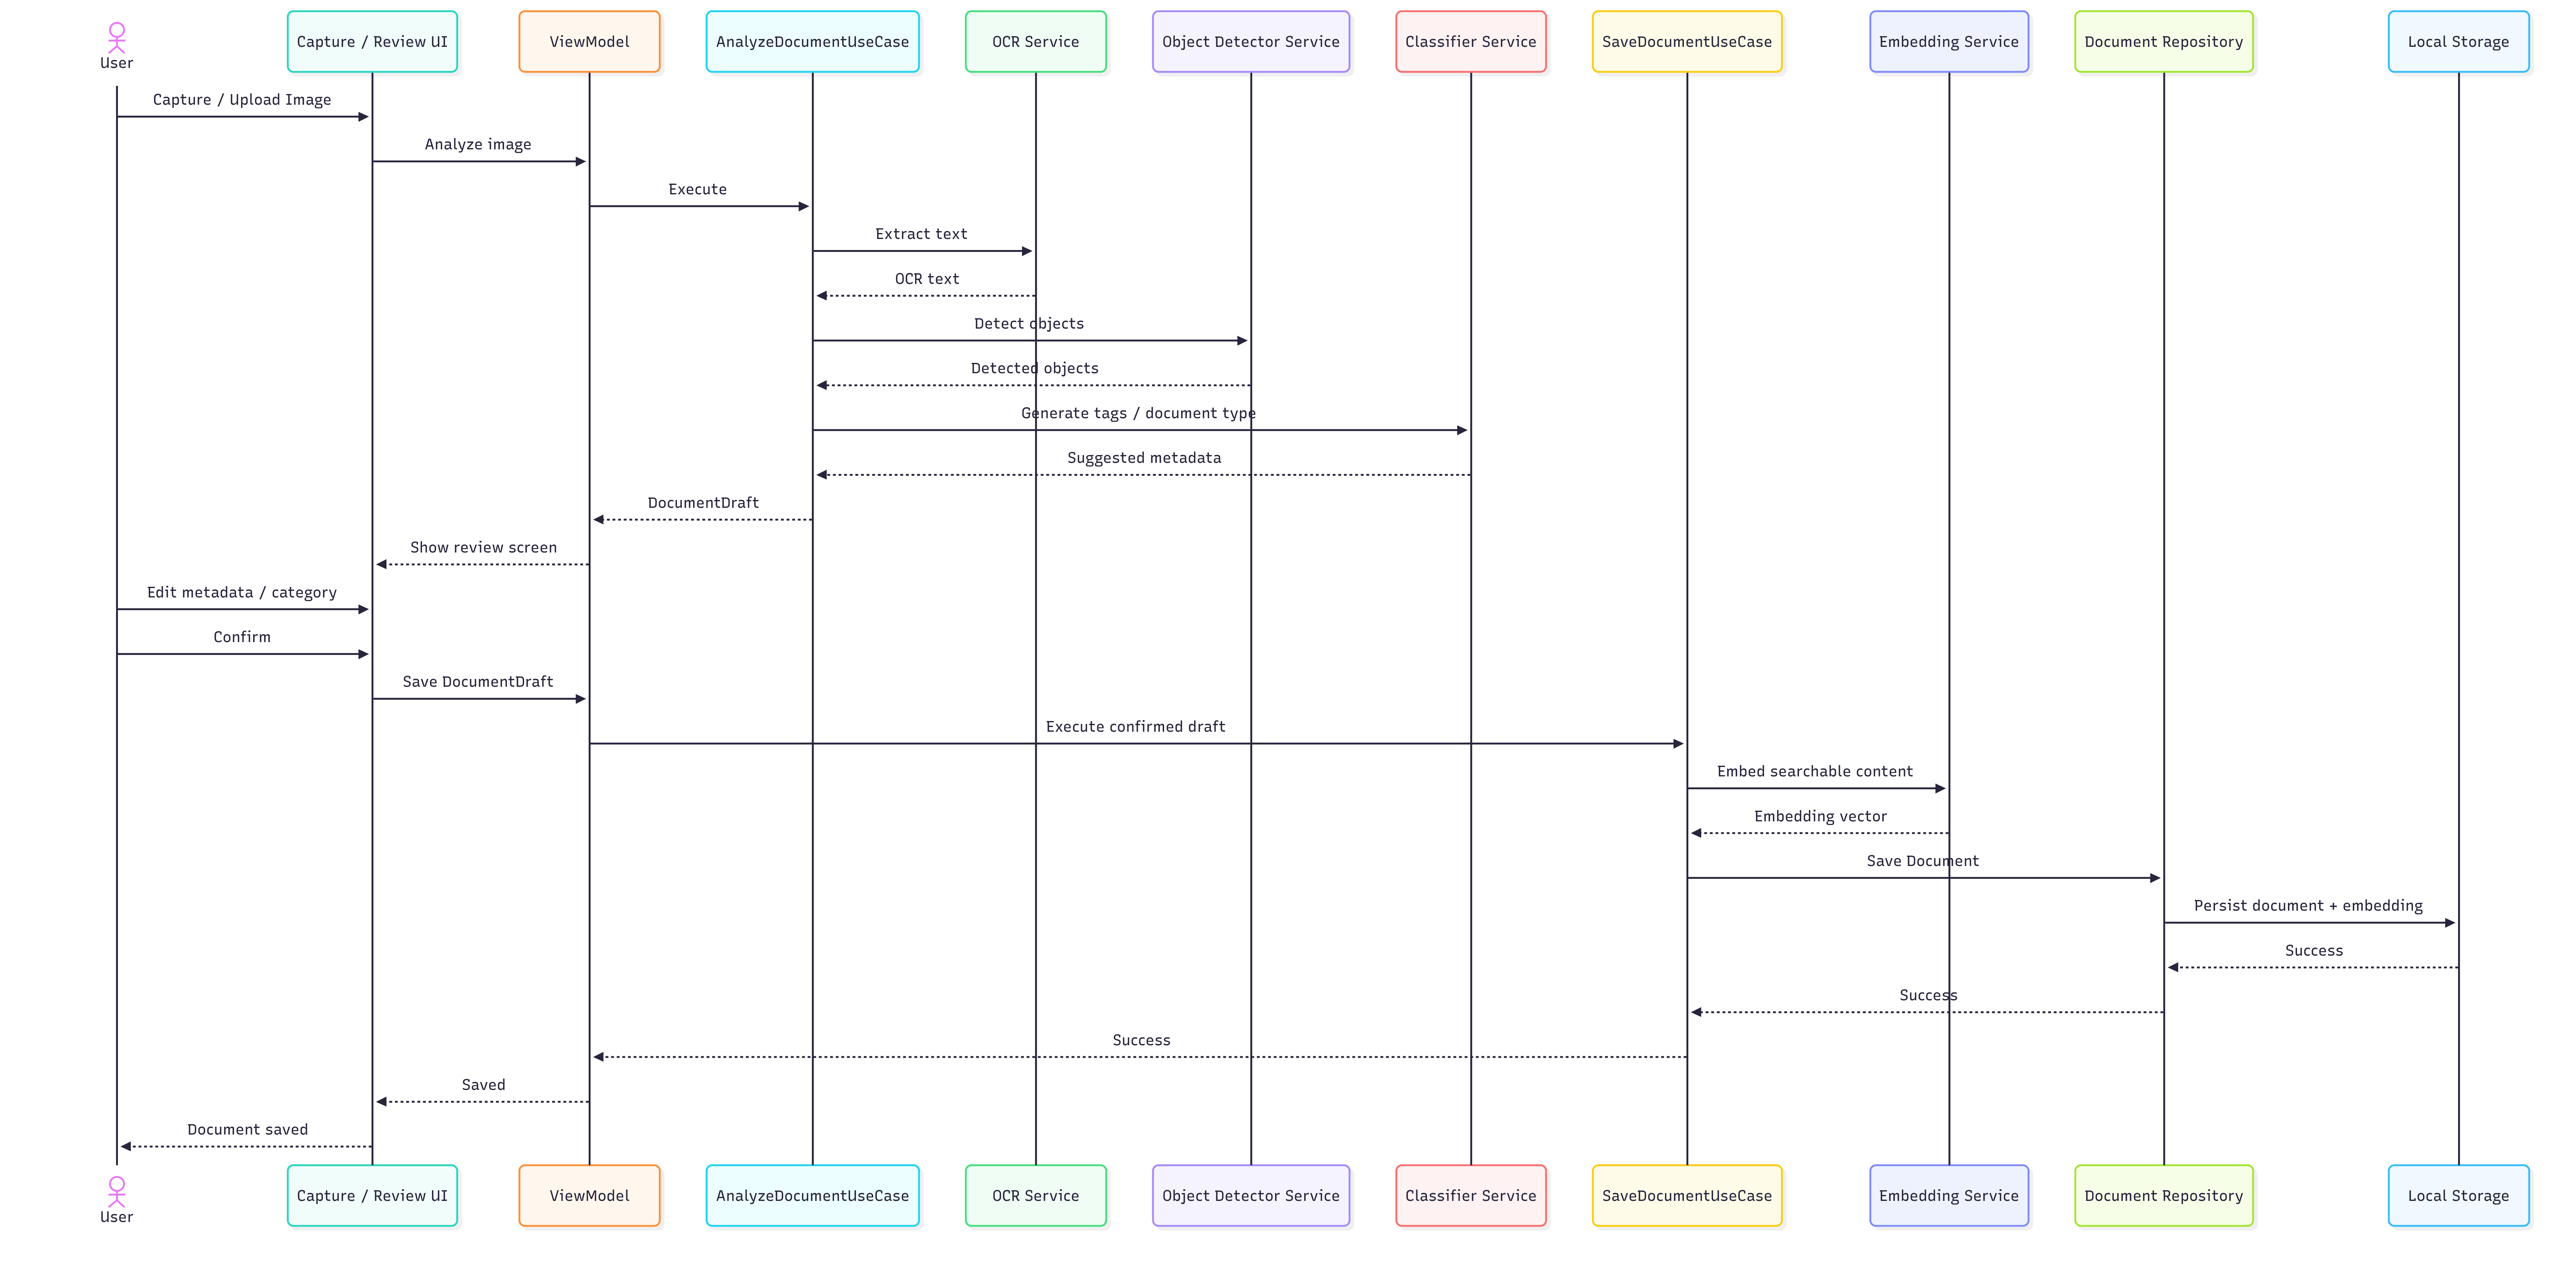
\includegraphics[width=\textwidth]{figures/AnalyzeFlow.png}
\caption{Document analysis flow}
\label{fig:seq_capture_save}
\end{figure}

\subsubsection{Hybrid Search Flow}
The sequence below traces a real-time search query from user keystroke debouncing to embedding generation, similarity ranking, and reactive UI updates:

\begin{figure}[H]
\centering
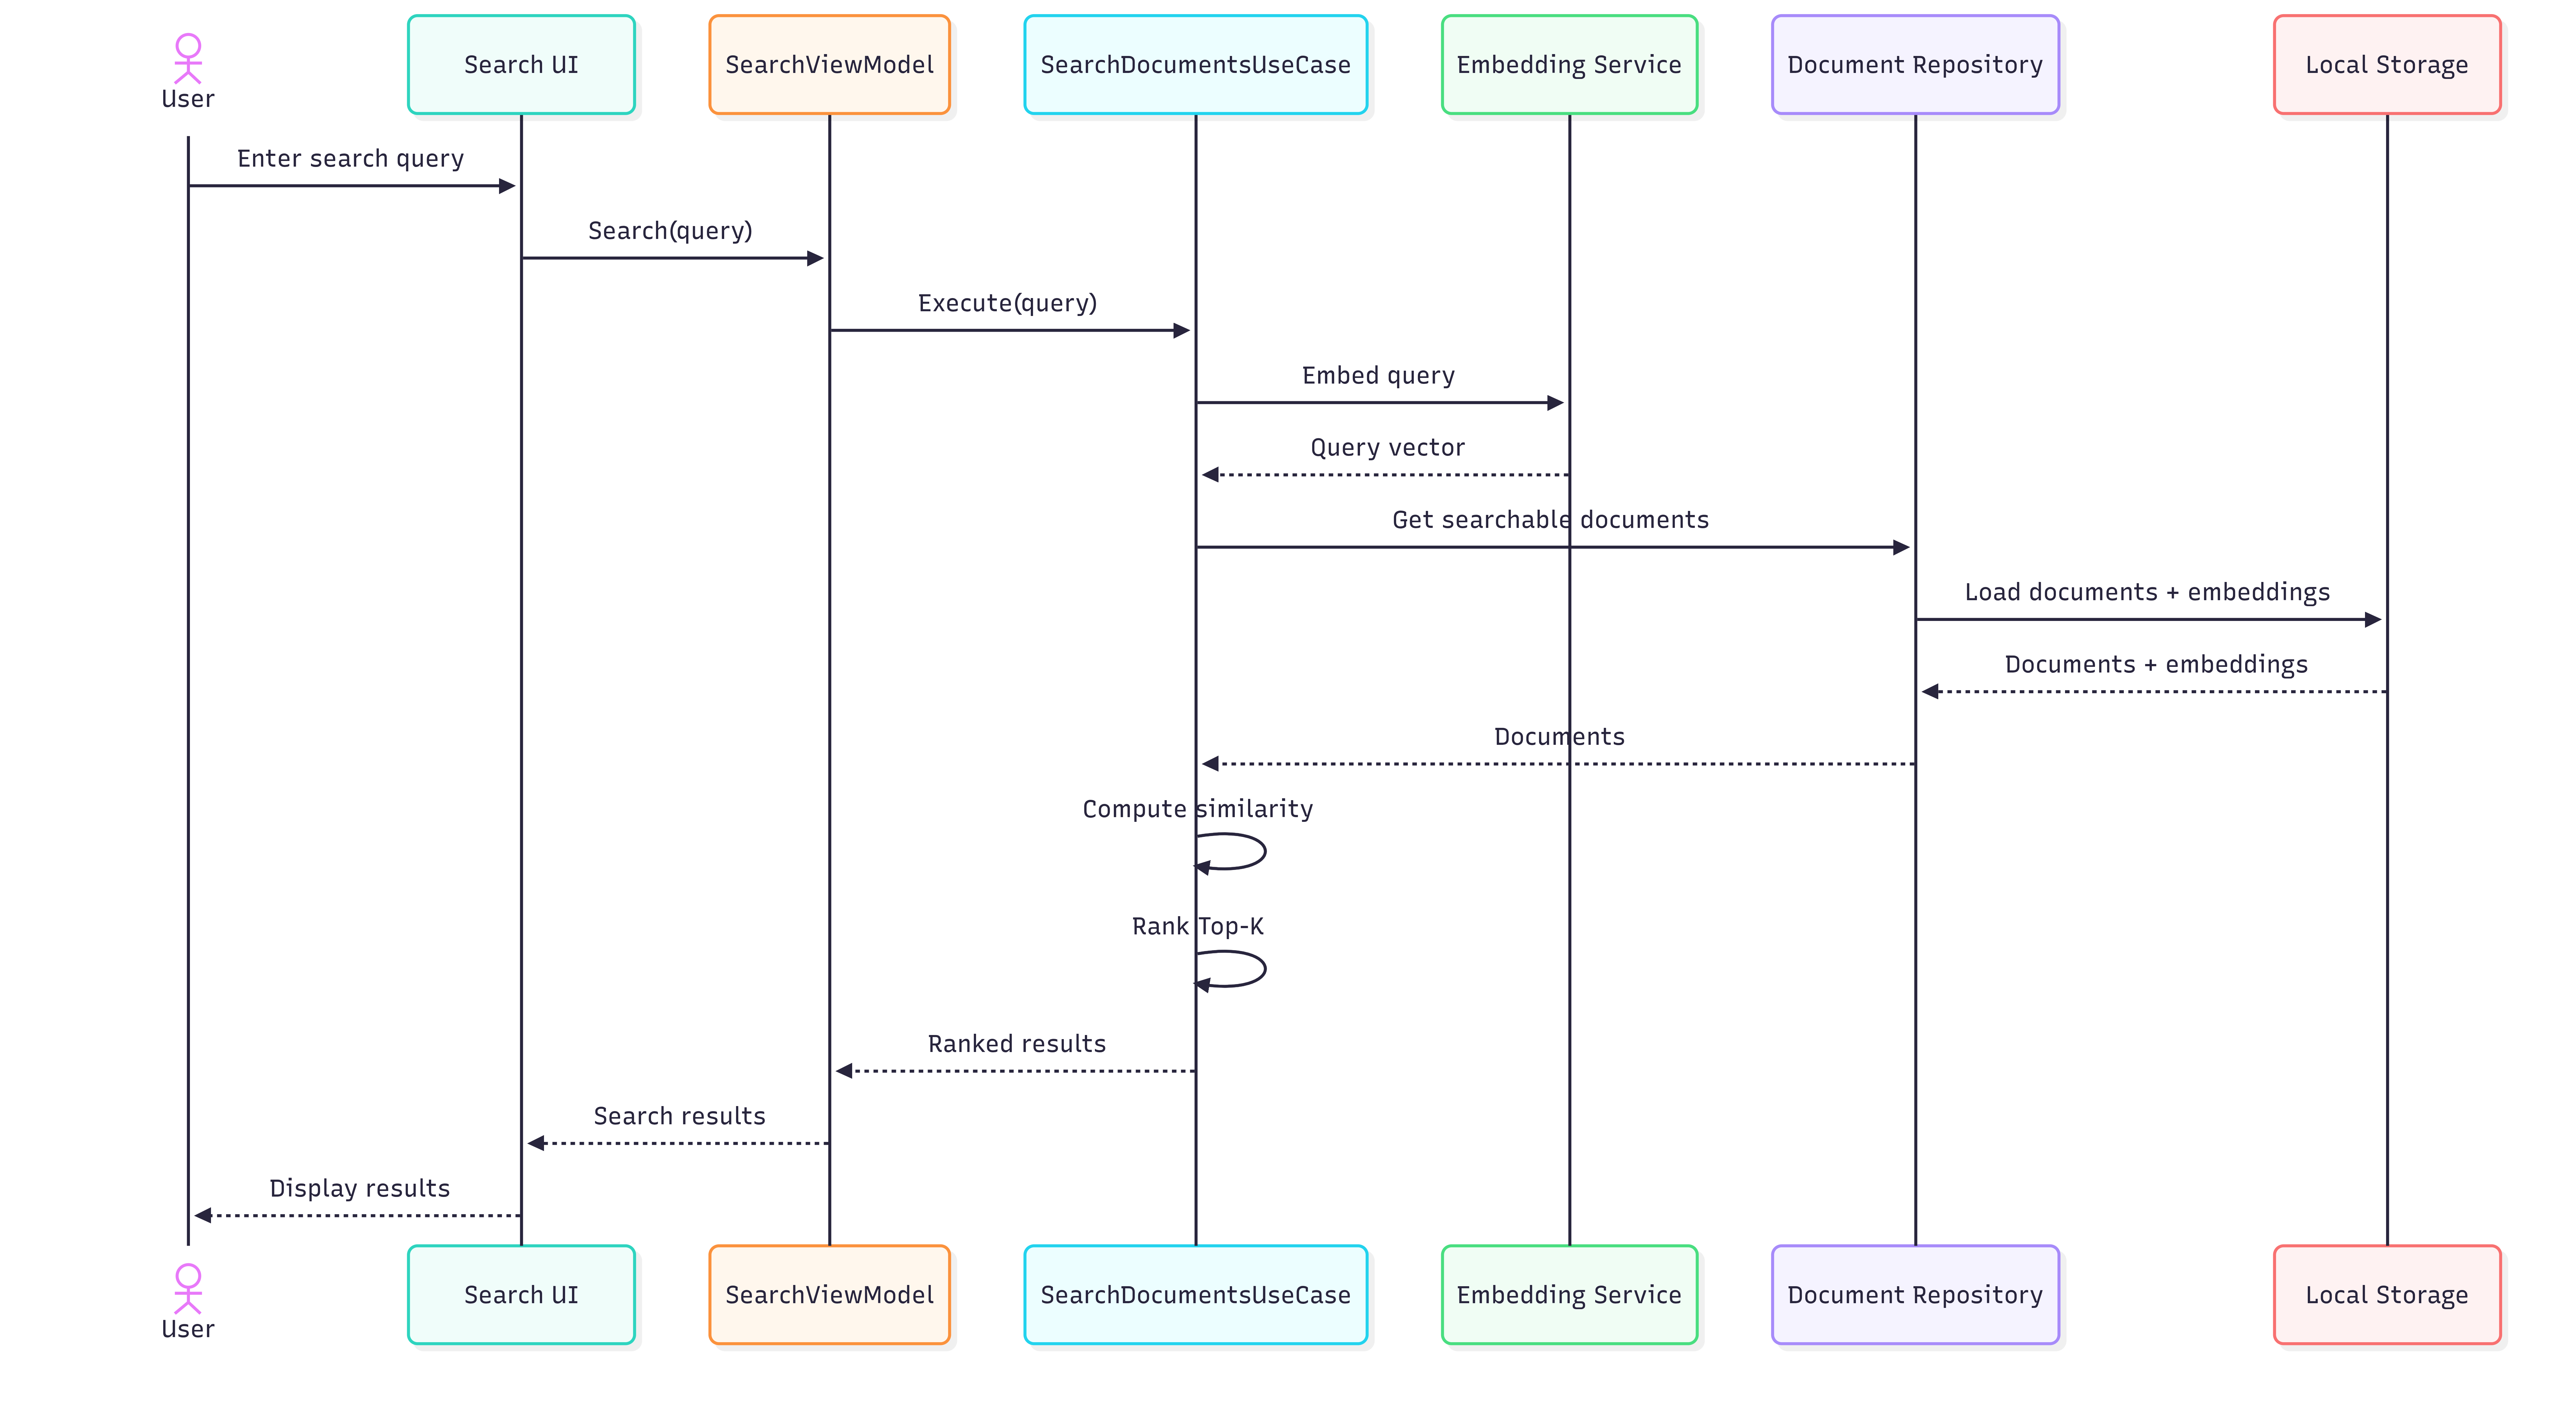
\includegraphics[width=\textwidth]{figures/SearchFlow.png}
\caption{Hybrid search flow}
\label{fig:seq_search}
\end{figure}

